\chapter{Control}
\label{chap:control}

\section{Overview of the control system}
This is an overview of the information flow for control in regard to the rest of the system containing, sensors, \ac{LLI} and \ac{HLI}.

\begin{figure}[htbp]
	\centering
	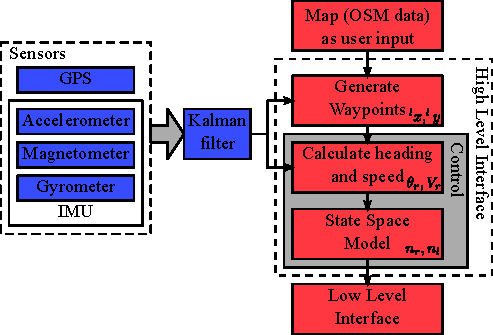
\includegraphics[width=\textwidth]{img/vessel-block-overview}
	\caption{Overview of control information flow in regard to the subsystems. The blue part indicates information that is not fetched directly to the control part, it is electrically connected to the \ac{LLI} whilst being forwarded to the \ac{HLI}.}
	\label{fig:vessel-block-overview}
\end{figure}

\todo{Illustrate on figure~\vref{fig:vessel-block-overview} where RF comms is or maybe that should be on the block overvieww diagram without regard to contorl abstraction}



\section{State Space Model}

%1. what is it
\todo{description}

%2. why are we using it


The reason for which the State Space representation was chosen is because it is a very simple, yet powerful way of modeling linear systems, allowing us to adjust and manipulate its dynamics in a very wide range of situations. 

%3. what are we using from it

\subsection{Linearizing the outputs}

Using Newton's second law of motion for forward  and rotational movement (F = m * A; T = I * W'), we can easily see that the inputs to our system will be F and T representing the forward force and the torque produced by the motors. It is worth mentioning that, since there are two propellers rotating in opposite directions, a torque that would induce a rotation around Z axis passing through the boat's center of mass only if the two propellers are rotating at different speeds.

These two rotational speeds N1 and N2 were initially included in the state space model as inputs to the system, as they could be controlled directly via a PWM pulse. This though proved to complicate matters because the relationship between the speeds of the propellers N1 and N2 and the force F and torque T generating accelerations is not a linear one. Because of this, our system would not be linear and would be beyond the scope of this project. 

\todo{insert formulas for [F, T] -> [n1, n2] transformation here}

In order to prevent this from happening, the state space model was updated to only calculate the force T and torque T necessary for driving and turning the ship, and this would keep our system linear. in order to transform from [T, F] to [N1, N2], another module was introduced in the system which would implement this non-linear function. 

This is a better solution anyway because if the state space model only outputs T and F, then it could be used for some other ship configurations, without modifications to the model, only to the module that translates the force and torque to N1 and N2. This, for example, can allow us to change the size of the propellers or their positions.

\subsection{Linearizing the drag forces}
\label{sect:Linearizing drag forces}

The drag forces acting on the bow of the ship while it's moving through the water are influenced by the area of the hull that is below water depth in the direction of movement, the density of the water, a drag constant $ C_{D} $ , and the square of the ship's speed components $ v_{x} $ and $ v_{y} $. 

A worthy note is the fact that the drag coefficient $ C_{D} $ will have two values depending on the direction of the ship's movement. When moving forward in the x direction, the coefficient $ C_{D}x $ will be approximated for a triangular shape, which is the closest simple shape that we have values for. For lateral movement in the y direction, $ C_{D}y $is given for a square box. These approximations should not present a problem in the operation of our control system as the errors ca easily be corrected and adjusted for by a good controller.

\[ D_{x}(v_{x}) = \frac{C_{Dx}\cdot\rho_{water}\cdot A_{front}\cdot v_{x}^{2}}{2} \]
\[ D_{y}(v_{y}) = \frac{C_{Dy}\cdot\rho_{water}\cdot A_{side}\cdot  v_{y}^{2}}{2} \]

Where $ D_{x}(v_{x}) $ and $ D_{y}(v_{y})$ are the drag forces dependent on the forward and lateral speeds respectively, $ \rho_{water} $ is the density of the water, $ A_{front} $ is the frontal area of the hull and $ A_{side} $ is the lateral area. 

The drag torque that is produced by the drag force acting on the hull of the ship, as the ship rotates through the water is dependent on the square of the angular velocity $ \omega $:

\[ \tau(\omega) = \frac{C_{D} \cdot \rho_{water} \cdot d \cdot (r_{f}^{4} + r_{b}^{4}) \cdot \omega^{2}}{8} \]

Where $ \tau(\omega) $ is the torque generated by the angular speed $ \omega $, $ d  $ is the depth of the ship that is submerged in water, $ r_{f} $ and $ r_{b} $ are the radii of the ship from the center of mass towards the front and back end, respectively.

These forces are obviously non-linear and thus cannot be integrated into the linear Kalman filter or State Space Model. Because we will usually use a constant speed it is feasible to linearize these forces for that value and not have big errors. The angular drag torque can also be linearized around a mean turning speed because the radii of the corners of the paths are also constant.

Approximation of the drag forces around the points of interest $v_{l} $ and $\omega_{l}$ is done using the first order term of the Taylor expansion:

\[ y_{l}(x) = f(a) + f'(a)(x-a) \]

Where $y = f(x)$ is the function we want to linearize around a value of interest $a$. Applying this formula to our situation yields:

\[ Dx_{l}(v_{x}) = \frac{C_{D}x\cdot\rho_{water}\cdot A_{front}\cdot v_{l}^{2}}{2} + (C_{D}x\cdot\rho_{water}\cdot A_{front})\cdot (v_{x}-v_{l}) \]

\[ Dy_{l}(v_{y}) = \frac{C_{Dy}\cdot\rho_{water}\cdot A_{side}\cdot v_{l}^{2}}{2} + (C_{D}y\cdot\rho_{water}\cdot A_{side})\cdot (v_{y}-v_{l}) \]

\[ \tau_{l}(\omega) = \frac{C_{D}y \cdot \rho_{water} \cdot d \cdot (r_{f}^{4} + r_{b}^{4}) \cdot \omega_{l}^{2}}{8} + \frac{C_{D}y \cdot \rho_{water} \cdot d \cdot (r_{f}^{4} + r_{b}^{4}) \cdot \omega_{l}}{4} \cdot (\omega - \omega_{l}) \] 

\begin{figure}[htbp]
	\centering
	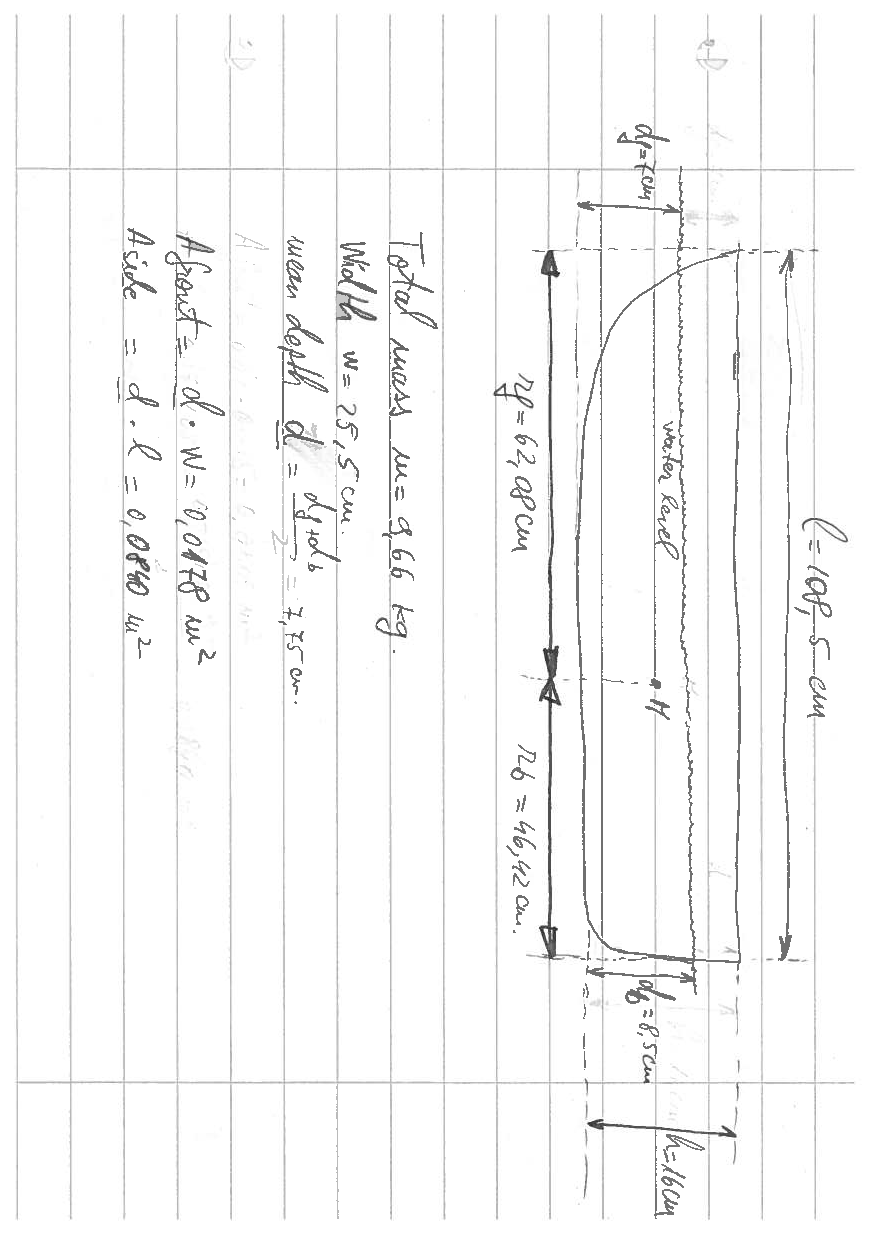
\includegraphics[width=\textwidth, trim=1.8cm 0cm 0cm 2cm, clip = true, angle = 90, width=\textwidth]{img/ship_sizes}
	\caption{Sketch of ship sizes as measured after the maiden voyage}
	\label{fig:ship_sizes}
\end{figure}

Given \vref{fig:ship_sizes}
 $ v_{l} = 1m/s $ ,
 $ \omega_{l} = 1 s ^{-1} $ ,
 $ C_{D}x = 0.5 $ (triangle) ,
 $ C_{D}y = 1 $ (box) ,
 $ \rho = 1000 kg/m ^{2} $,
 $ A_{front} = 0.0178 m^{2} $,
 $ A_{side} = 0.0840 m ^{2} $,
 $ d = 0.0775 m $,
 $ r_{f} = 0.6208 m $,
 $ r_{b} = 0.4642 m $,
the linearized formulas for the drag forces can be computed to be:


\begin{align}
 Dx_{l}(v) &= -4.45 + 8.9 \cdot v_{x} \\
 Dy_{l}(v) &= -42 + 84 \cdot v_{y} \\
 \tau_{l}(\omega) &= -1.88 + 3.77 \cdot \omega
\end{align}

From which we can identify the coefficients that correspond tot the linear relation $ y_{l}(x) = \alpha + \beta \cdot x $:\\
\begin{minipage}{0.3\linewidth}
\[ \alpha_{x} = -4.45 \] 
\[ \beta_{x} = 8.9 \]
\end{minipage}
\begin{minipage}{0.3\linewidth}
\[ \alpha_{y} = -42 \] 
\[ \beta_{y} = 84 \]
\end{minipage}
\begin{minipage}{0.3\linewidth}
\[ \alpha_{\omega} = -1.88 \]
\[ \beta_{\omega} = 3.77 \]
\end{minipage}


\subsection{Choosing the right states}

The variables we chose to be the states in our model are the speed of the ship in the forward direction in the ship frame $v$, the angular position of the ship's x axis relative to true North $\theta$ and the angular speed $\omega$.\\
\[\begin{cases}
F - F_{D} = m \cdot \dot{v}\\
T - T_{D} = I \cdot \dot{\omega}\\
\end{cases}\]

Where $ F $ and $ T $ are the force and torque produced by the propellers, $ F_{D} $ and $ T_{D} $ are the force and torque caused by water drag, $ m $ is the mass of the ship, $ I $ is the moment of inertia, $ \dot{v} $  and $ \dot{\omega} $ are forward and angular acceleration respectively.

The linearized drag force and torque from \ref{sect:Linearizing drag forces} can be substituted in these equations:
\begin{align}
 \dot{v} &= - \frac{\beta_{x} \cdot v}{m} + \frac{F}{m}\\
 \dot{\omega} &= - \frac{\beta_{y} \cdot \omega}{I} + \frac{T}{I}\\
 \dot{\theta} &= \omega
\end{align}

Note that we have also dropped the $ \alpha $ term of the equations because we're currently only interested in the dynamic behavior of the system. The $ \alpha $ offset will be compensated for when removing the steady state error. Consequently, these relations can be rewritten in a matrix notation as follows:
\[
\dot{
	\begin{bmatrix}
	 v\\
	 \theta\\
	 \omega
	\end{bmatrix}
}
=
\begin{bmatrix}
 -\frac{\beta_{x}}{m} & 0 & 0\\
 0 & 0 & 1\\
 0 & 0 & - \frac{\beta_{y}}{I}\\
\end{bmatrix}
\cdot
\begin{bmatrix}
v\\
\theta\\
\omega
\end{bmatrix}
+
\begin{bmatrix}
\frac{1}{m} & 0\\
0 & 0\\
0 & \frac{1}{I}\\
\end{bmatrix}
\cdot
\begin{bmatrix}
F\\
T
\end{bmatrix}
\]

This corresponds to the State Space Model equation:
\[\dot{X} = AX + BU\]

Since the output matrix we need is $ Y = \begin{bmatrix}v \\ \theta \end{bmatrix} $, the output equation
\[Y = CX + DU\]
becomes:
\[\begin{bmatrix}v \\ \theta \end{bmatrix}
 = 
\begin{bmatrix}
1 & 0\\
0 & 1\\
0 & 0
\end{bmatrix}
\cdot
\begin{bmatrix}
v\\
\theta\\
\omega
\end{bmatrix}
\]

So the system matrices are:
\[
A =\begin{bmatrix}
 -\frac{\beta_{x}}{m} & 0 & 0\\
 0 & 0 & 1\\
 0 & 0 & - \frac{\beta_{y}}{I}\\
\end{bmatrix}\\
B = \begin{bmatrix}
\frac{1}{m} & 0\\
0 & 0\\
0 & \frac{1}{I}\\
\end{bmatrix}\\
C = 
\begin{bmatrix}
1 & 0\\
0 & 1\\
0 & 0
\end{bmatrix}\\
D = 0
\]

\subsection{Discretizing for use with a particular timestep}

The system described so far is continuous and needs to be discretized before implementation in a computer algorithm, so we use the function c2d from MATLAB and the time step Ts in order to do this. \todo{explain more about c2d or what we will eventually use}

\subsection{Pole assignment}

For assigning poles, we use the lqr function implemented in MATLAB. This calculates the gain matrix $ F $ by minimizing the quadratic cost function:\todo{taken from here http://www.mathworks.se/help/control/ref/lqr.html}
\[
J(u)=\sum_{0}^{\inf} \{x^{T}Qx+u^{T}Ru+2x^{T}Nu\}
\]


\subsection{Reference gain}

A reference gain is calculated and implemented in order to counter the steady state error. This is calculated using the formula $ N = Nu+FNx $ \todo{insert refference to feedback book, page 470}, where:
\[
\begin{bmatrix}
Nx\\
Nu
\end{bmatrix}
=
\begin{bmatrix}
A & B\\
C & D
\end{bmatrix}^{-1}
\!
\cdot
\begin{bmatrix}
0\\
I
\end{bmatrix}
\]
\todo{Why we chose a lot of states in the beginning, and then were left with just a few?}
